\documentclass{article}
%\documentclass[fleqn]{article}

\marginparwidth 0.5in 
\oddsidemargin 0.25in 
\evensidemargin 0.25in 
\marginparsep 0.25in
\topmargin 0.25in 
\textwidth 6in \textheight 8 in

\usepackage[utf8]{inputenc}
\usepackage[T1]{fontenc}
\usepackage{ngerman}
\usepackage{graphics}
\usepackage{pdfpages} 
\usepackage{amsmath}

\title{Künstliche Intelligenz\\~\\Hausaufgabe 5\\ \small{N. Lehmann, T. Gleißner, A. Zubarev}}
\date{27.05.2015}

\begin{document}

\maketitle

%%%%%%%%%%%%%%%%%%%%%%%%%%%%%%%%%%%%%%%%%%%%%%%%%%%%%%%%%%%%%%%%%%%%%%%%%%%%%%%%%%%%%%%%%%%%%%
\section*{Aufgabe 1: Unifikation}
%%%%%%%%%%%%%%%%%%%%%%%%%%%%%%%%%%%%%%%%%%%%%%%%%%%%%%%%%%%%%%%%%%%%%%%%%%%%%%%%%%%%%%%%%%%%%%
Um die Disagreement Sets und den Most General Unifier zu finden, sucht man sich immer das linkste Symbol, bei dem sich die Formeln unterscheiden und bildet daraus ein Disagreement Set $S_i$ sowie Ersetzungsregeln $\sigma_i$. Anschließend wendet man die Ersetzungsregeln $\sigma_i$ auf die Formeln $S_i$ an, um die neuen Formeln $S_{i+1}$ zu erhalten bis entweder die Formeln gleich sind oder man feststellt, dass Unifikation nicht möglich ist.

\begin{flalign*}
S_0 &= \{p(X,f(Y),Z), p(T,T,g(cat)), p(f(dog),S,g(W))\} \\
D_0 &= \{X,T,f(dog)\} \\
\sigma_0 &= \{X/f(dog), T/f(dog)\} \\
S_1 &= \{p(f(dog),f(Y),Z), \; p(f(dog),f(dog),g(cat)), \; p(f(dog),S,g(W))\} \\
D_1 &= \{f(Y), f(dog), S\} \\
% muesste es hier nicht {Y,dog,S} sein? f( ist ja gleich..?
\sigma_1 &= \{X/f(dog), T/f(dog), Y/dog, S/f(dog)\} \\
S_2 &= \{p(f(dog),f(dog),Z), \; p(f(dog),f(dog),g(cat)), \; p(f(dog),f(dog),g(W))\} \\
D_2 &= \{Z,g(cat),g(W)\} \\
% muesste es hier nicht {Z,cat,W} sein? g( ist ja gleich..?
\sigma_2 &= \{X/f(dog), T/f(dog), Y/dog, S/f(dog), Z/g(cat), W/cat\} \\
S_3 &= \{p(f(dog), f(dog), g(cat)), \; p(f(dog), f(dog), g(cat)), \; p(f(dog), f(dog), g(cat))\}
% Warum taucht in S_3 p(f(dog), f(dog), g(cat)) zweimal auf?
\end{flalign*}

Alle Terme in $S_3$ sind gleich, das Most General Unifier ist damit
\begin{equation*}
\sigma_2 = \{X/f(dog), T/f(dog), Y/dog, S/f(dog), Z/g(cat), W/cat\}
\end{equation*}
\newpage
%%%%%%%%%%%%%%%%%%%%%%%%%%%%%%%%%%%%%%%%%%%%%%%%%%%%%%%%%%%%%%%%%%%%%%%%%%%%%%%%%%%%%%%%%%%%%%
%%%%%%%%%%%%%%%%%%%%%%%%%%%%%%%%%%%%%%%%%%%%%%%%%%%%%%%%%%%%%%%%%%%%%%%%%%%%%%%%%%%%%%%%%%%%%%
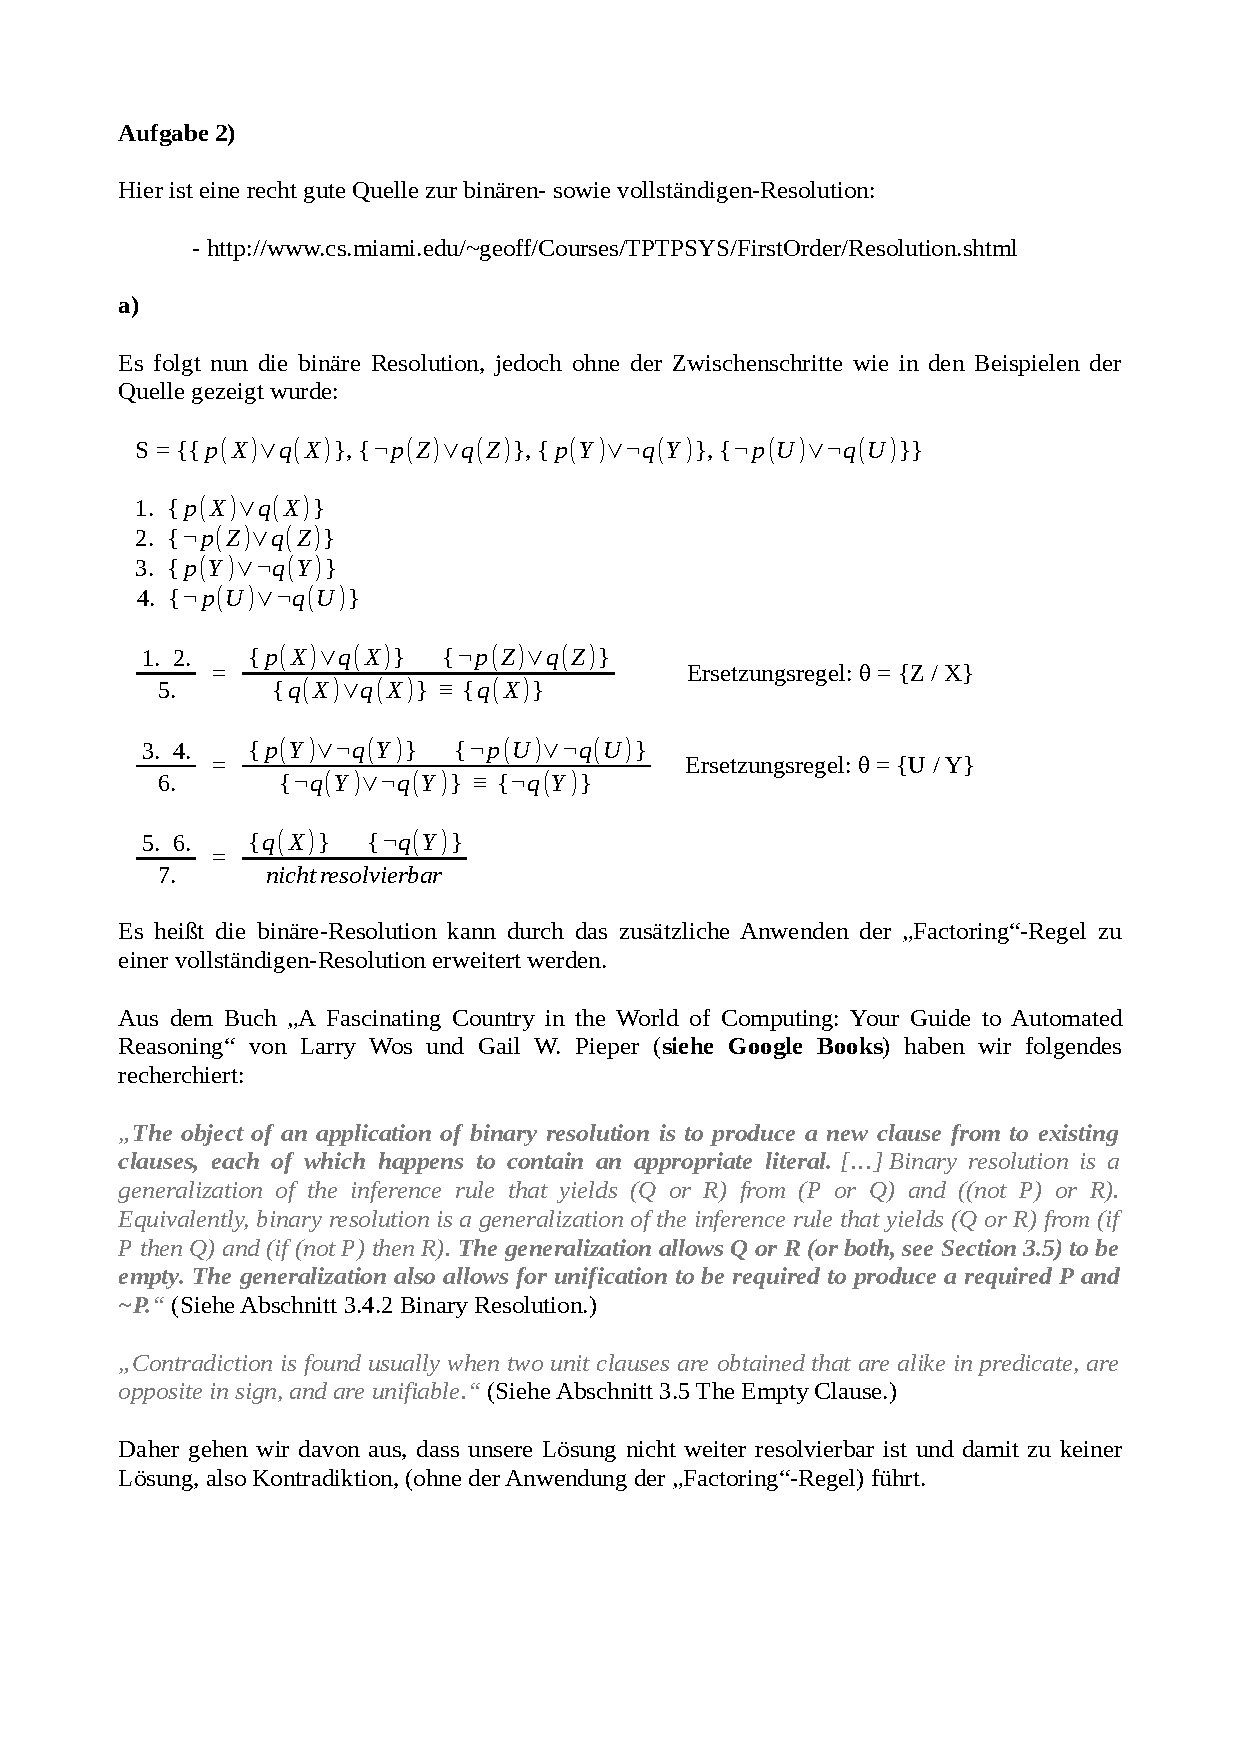
\includepdf[pages=1]{ki_hw_05_2a.pdf}

\subsection*{Aufgabe 2b: Full Resolution}

% Muss hier eine Vorbverarbeitung stattfinden?
$S = \{ p(X) | q(X) , \sim p(Z) | q(Z) , p(Y) | \sim q(Y) , \sim p(U) | \sim q(U) \}$\\
\\
$CNF = p(X) \vee q(X) \wedge \neg p(Z) \vee q(Z) \wedge p(Y) \vee \neg q(Y) \wedge \neg p(U) \vee \neg q(U)$\\
\\
$\neg CNF = \neg p(X) \wedge \neg q(X) \vee p(Z) \wedge \neg q(Z) \vee \neg p(Y) \wedge q(Y) \vee p(U) \wedge q(U)$\\
\\
$\neg CNF = \underbrace{(\neg p \wedge \neg q)}_{1} \vee \underbrace{(p \wedge \neg q)}_{2} \vee \underbrace{(\neg p \wedge q)}_{3} \vee \underbrace{(p \wedge q)}_{4}$\\
\\
Vollständige Resolution:\\
\\
$1+2+4 = 5 = \neg q \wedge q = \emptyset$\\
\newpage

%%%%%%%%%%%%%%%%%%%%%%%%%%%%%%%%%%%%%%%%%%%%%%%%%%%%%%%%%%%%%%%%%%%%%%%%%%%%%%%%%%%%%%%%%%%%%%
\section*{Aufgabe 3: CNF-Resoluton}
%%%%%%%%%%%%%%%%%%%%%%%%%%%%%%%%%%%%%%%%%%%%%%%%%%%%%%%%%%%%%%%%%%%%%%%%%%%%%%%%%%%%%%%%%%%%%%

Umwandeln der Klausel $(A1 \land A2 \land A3) \Rightarrow B$

Simplify
\begin{equation*}
\begin{aligned}
\lnot (( \forall X (\lnot p(X) \lor ( \forall Y ( \lnot k(Y) \lor \lnot m(X,Y))))) \land \\
(\forall X ( \lnot p(X) \lor ( \exists Y ( f(Y) \land m(X,Y)))) ) \land \\
(\exists X (p(X)))) \lor \\
( \exists X (f(X) \land \lnot k(X)) )
\end{aligned}
\end{equation*}

Move negations in
\begin{equation*}
\begin{aligned}
(\lnot ( \forall X (\lnot p(X) \lor ( \forall Y ( \lnot k(Y) \lor \lnot m(X,Y))))) \lor \\
\lnot (\forall X ( \lnot p(X) \lor ( \exists Y ( f(Y) \land m(X,Y)))) ) \lor \\
\lnot (\exists X (p(X)))) \lor \\
( \exists X (f(X) \land \lnot k(X)) )
\end{aligned}
\end{equation*}
\begin{equation*}
\begin{aligned}
(\exists X \lnot (\lnot p(X) \lor ( \forall Y ( \lnot k(Y) \lor \lnot m(X,Y)))) \lor \\
\exists X \lnot ( \lnot p(X) \lor ( \exists Y ( f(Y) \land m(X,Y)))) \lor \\
\forall X \lnot (p(X))) \lor \\
( \exists X (f(X) \land \lnot k(X)) )
\end{aligned}
\end{equation*}
\begin{equation*}
\begin{aligned}
(\exists X ( \lnot \lnot p(X) \land \lnot ( \forall Y ( \lnot k(Y) \lor \lnot m(X,Y)))) \lor \\
\exists X ( \lnot \lnot p(X) \land \lnot ( \exists Y ( f(Y) \land m(X,Y)))) \lor \\
\forall X \lnot (p(X))) \lor \\
( \exists X (f(X) \land \lnot k(X)) )
\end{aligned}
\end{equation*}
\begin{equation*}
\begin{aligned}
(\exists X ( p(X) \land ( \exists Y \lnot ( \lnot k(Y) \lor \lnot m(X,Y)))) \lor \\
\exists X ( p(X) \land ( \forall Y \lnot ( f(Y) \land m(X,Y)))) \lor \\
\forall X \lnot (p(X))) \lor \\
( \exists X (f(X) \land \lnot k(X)) )
\end{aligned}
\end{equation*}
\begin{equation*}
\begin{aligned}
(\exists X ( p(X) \land ( \exists Y ( k(Y) \land m(X,Y)))) \lor \\
\exists X ( p(X) \land ( \forall Y ( \lnot f(Y) \lor \lnot m(X,Y)))) \lor \\
\forall X \lnot (p(X))) \lor \\
( \exists X (f(X) \land \lnot k(X)) )
\end{aligned}
\end{equation*}

Move quantifiers out
\begin{equation*}
\begin{aligned}
(\exists A \exists B ( p(A) \land ( k(B) \land m(A,B))) \lor \\
\exists C \forall D ( p(D) \land ( \lnot f(D) \lor \lnot m(C,D))) \lor \\
\forall E \lnot (p(E))) \lor \\
( \exists F (f(F) \land \lnot k(F)) )
\end{aligned}
\end{equation*}
\begin{equation*}
\begin{aligned}
\exists A \exists B \exists C \forall D \forall E \exists F \\
( ( p(A) \land ( k(B) \land m(A,B))) \lor \\
 ( p(D) \land ( \lnot f(D) \lor \lnot m(C,D))) \lor \\
 \lnot (p(E)) \lor \\
(f(F) \land \lnot k(F)) )
\end{aligned}
\end{equation*}

Skolemize
\begin{equation*}
\begin{aligned}
\gamma = \{\} \\
\exists A: A/sk_A(\{\}) \\
\exists B: B/sk_B(\{\}) \\
\exists C: C/sk_C(\{\}) \\
\forall D: \gamma = \{D\} \\
\forall E: \gamma = \{D,E\} \\
\exists F: F/sk_F(\{D,E\})
\end{aligned}
\end{equation*}
\begin{equation*}
\begin{aligned}
(( p(sk_A(\{\})) \land ( k(sk_B(\{\})) \land m(sk_A(\{\}),sk_B(\{\})))) \lor \\
( p(D) \land ( \lnot f(D) \lor \lnot m(sk_C(\{\}),D))) \lor \\
\lnot (p(E)) \lor \\
(f(sk_F(\{D,E\})) \land \lnot k(sk_F(\{D,E\}))) )
\end{aligned}
\end{equation*}

Distribute disjunctions and Convert to CNF
\newline
Zu viele Zeilen, wahrscheinlich ist auch irgendwo ein Fehler drinnen, Teilaufgabe b ist damit dann auch schlecht zu lösen...

%%%%%%%%%%%%%%%%%%%%%%%%%%%%%%%%%%%%%%%%%%%%%%%%%%%%%%%%%%%%%%%%%%%%%%%%%%%%%%%%%%%%%%%%%%%%%%
\section*{Aufgabe 4: Occures Check}
%%%%%%%%%%%%%%%%%%%%%%%%%%%%%%%%%%%%%%%%%%%%%%%%%%%%%%%%%%%%%%%%%%%%%%%%%%%%%%%%%%%%%%%%%%%%%%
Der Occurs Check in SWI Prolog wird mit der Funktion $unifiy\_with\_occurs\_check(operand_1,operand_2)$ aktiviert.

\vbox{
Ohne Occurs Check:
\begin{verbatim}
?- A=f(A).
A = f(A).
?- A.
% ... 1,000,000 ............ 10,000,000 years later
% 
%       >> 42 << (last release gives the question)
\end{verbatim}
}

\vbox{
Mit Occurs Check:
\begin{verbatim}
?- unify_with_occurs_check(A,f(A)).
false.
\end{verbatim}
}

\end{document}